%; whizzy paragraph -pdf xpdf -latex ./whizzypdfptex.sh
%; whizzy-paragraph "^\\\\begin{frame}\\|\\\\emtext"
% latex beamer presentation.
% platex, latex-beamer でコンパイルすることを想定。 

%     Tokyo Debian Meeting resources
%     Copyright (C) 2012 Junichi Uekawa

%     This program is free software; you can redistribute it and/or modify
%     it under the terms of the GNU General Public License as published by
%     the Free Software Foundation; either version 2 of the License, or
%     (at your option) any later version.

%     This program is distributed in the hope that it will be useful,
%     but WITHOUT ANY WARRANTY; without even the implied warreanty of
%     MERCHANTABILITY or FITNESS FOR A PARTICULAR PURPOSE.  See the
%     GNU General Public License for more details.

%     You should have received a copy of the GNU General Public License
%     along with this program; if not, write to the Free Software
%     Foundation, Inc., 51 Franklin St, Fifth Floor, Boston, MA  02110-1301 USA

\documentclass[cjk,dvipdfmx,12pt]{beamer}
\usetheme{Tokyo}
\usepackage{monthlypresentation}

%  preview (shell-command (concat "evince " (replace-regexp-in-string "tex$" "pdf"(buffer-file-name)) "&")) 
%  presentation (shell-command (concat "xpdf -fullscreen " (replace-regexp-in-string "tex$" "pdf"(buffer-file-name)) "&"))
%  presentation (shell-command (concat "evince " (replace-regexp-in-string "tex$" "pdf"(buffer-file-name)) "&"))

%http://www.naney.org/diki/dk/hyperref.html
%日本語EUC系環境の時
\AtBeginDvi{\special{pdf:tounicode EUC-UCS2}}
%シフトJIS系環境の時
%\AtBeginDvi{\special{pdf:tounicode 90ms-RKSJ-UCS2}}

\title{東京エリアDebian勉強会}
\subtitle{第95回 2012年12月度}
\author{上川純一\\dancer@debian.org}
\date{2012年12月15日}
\logo{
\includegraphics[width=8cm]{image200607/openlogo-light.eps}}

\begin{document}

\frame{\titlepage{}}

\begin{frame}{設営準備にご協力ください。}
会場設営よろしくおねがいします。
\end{frame}

\begin{frame}{Agenda}
\begin{minipage}[t]{0.45\hsize}
  \begin{itemize}
  \item 注意事項
	\begin{itemize}
	 \item 飲食禁止
	 \item 宗教禁止
	 \item 営利活動禁止
	\end{itemize}
   \item 最近あったDebian関連のイベント報告
	\begin{itemize}
        \item 第94回 東京エリアDebian勉強会
	\end{itemize}
   \item 事前課題紹介
 \end{itemize}
\end{minipage} 
\begin{minipage}[t]{0.45\hsize}
 \begin{itemize}
  \item im-config 
  \item 著作権法改正
  \item 2012年のDebian勉強会を振り返る
 \end{itemize}
\end{minipage}
\end{frame}

\emtext{事前課題}
{\footnotesize
 %; whizzy-master ../debianmeetingresume201212.tex
% $B0J>e$N@_Dj$r$7$F$$$k$?$a!"$3$N%U%!%$%k$G(B M-x whizzytex $B$9$k$H!"(B
% whizzytex$B$,MxMQ$G$-$^$9(B

\begin{prework}{ $B5HLn(B(yy\_y\_ja\_jp) }

\preworksection{DFSG$B$K$*$$$F$N<+M3$K$D$$$FO@$8$F$/$@$5$$!#(B}

 $B<+M3$r<i$k$?$a$N@)8B$G$"$k!#(B

\preworksection{Debian$B$K4X$7$F!"#2#0#1#2G/$r$U$j$+$($C$F#2#0#1#3G/$d$C$F$*$-$?$$$3$H$rO@$8$F$/$@$5$$!#(B}

 Bug squashing$B!$(BDDTP$B$J$I$G$NK]Lu(B
\end{prework}

\begin{prework}{ seiji-n }
\preworksection{DFSG$B$K$*$$$F$N<+M3$K$D$$$FO@$8$F$/$@$5$$!#(B}

5.$B$9$Y$F$N8D?M!"CDBN$NJ?Ey(B

6.$B%i%$%;%s%9$O!"$9$Y$F$N8D?M$dCDBN$r:9JL$7$F$O$J$j$^$;$s!#(B

DFSG$B$N>e5-3F>r9`$K4X$7$F!"%F%m%j%9%HEyH?<R2qCDBN$dHH:a<T!"HH:a=8CD$K$h$k(B
$BH?<R2qE*3hF0!"HH:a9T0Y$X$NMxMQ$KBP$7$F!":9JL$G$O$J$/$H6hJL$O$7$F$*$j!"(B
($B5,@)$O$G$-$J$$$J$,$i$b(B)$B7h$7$FA4LLE*$K>5G'$7$F$$$kLu$G$O$J$$$H$$$&(B
$B0U;VI=L@E*$J;v$r$9$Y$-$G$O$J$$$+!#$J$<$7$J$$$N$+!#$=$N>e$G$N<+M3$G$O(B
$B$J$$$+$H9M$($F$$$^$9!#(B


$BL\I8J,Ln$NJ?Ey(B

\preworksection{Debian$B$K4X$7$F!"#2#0#1#2G/$r$U$j$+$($C$F#2#0#1#3G/$d$C$F$*$-$?$$$3$H$rO@$8$F$/$@$5$$!#(B}

$B62=L$G$9$,(B2012$BG/$O(BDebian$B$K4X$7$F2?$b$7$F$$$^$;$s!#$3$l$+$i3X$s$G9T$-$?$$$H;W$$$^$9!#(B

\end{prework}

\begin{prework}{ dictoss($B?yK\!!E5=<(B) }

\preworksection{DFSG$B$K$*$$$F$N<+M3$K$D$$$FO@$8$F$/$@$5$$!#(B}

$B#9HVL\$N!V%i%$%;%s%9$OB>$N%=%U%H%&%'%"$r?/32$7$J$$!W$H$"$k!#(BLGPL$B%i%$%;%s%9$O(BGFSG$B8_49%i%$%;%s%9$@$,<B9T;~$OB>$N%=%U%H%&%'%"$N<+M3$r?/32$7$F$k>l9g$,$"$j$=$&$J5$$,$9$k$,$I$&$J$s$@$m$&$+!#(B


\preworksection{Debian$B$K4X$7$F!"#2#0#1#2G/$r$U$j$+$($C$F#2#0#1#3G/$d$C$F$*$-$?$$$3$H$rO@$8$F$/$@$5$$!#(B}

$B:#G/$O(Barmel$B%"!<%-%F%/%A%c$N(Bdebian$B$r=i$a$F<+J,$G%$%s%9%H!<%k$7$F$_$?!#@h?MC#$NCN7C$,$"$k$?$a3d$H$9$s$J$jF~$C$F$7$^$C$F(Bdebian$B$O$9$4$$$H;W$C$?!#MhG/$O(Bmips$B7O$N%O!<%I$rC5$7$F(Bdebian$B$rF~$l$F?'!9;n$7$F$_$?$$$H;W$$$^$9!#(B
\end{prework}

\begin{prework}{ $B%-%?%O%i(B }
\preworksection{DFSG$B$K$*$$$F$N<+M3$K$D$$$FO@$8$F$/$@$5$$!#(B}

 $BO@$8$kDx$NCNG=$O$J$$$N$G!"BX$o$j$K46A[$r!#(B
$BB>$N%i%$%;%s%9Ey$KHf$Y!"4V8}$,9-$/!"8=<BE*$G!"@)8B$,>/$J$/!"(B
$B3+H/<T$N$_$J$i$:MxMQ<T$K$b?4CO$N$h$$<+M3$G$"$k$H;W$&!#(B

\preworksection{Debian$B$K4X$7$F!"#2#0#1#2G/$r$U$j$+$($C$F#2#0#1#3G/$d$C$F$*$-$?$$$3$H$rO@$8$F$/$@$5$$!#(B}
 $B;d;v$G$9$,!"0[F0$G;H$($J$/$J$C$?(BDebian$B<RFb%5!<%P$NBe$o$j$r2?$H$+$7$?$$$G$9$M!#(B
\end{prework}

\begin{prework}{ $B@P0f0lIW(B }

\preworksection{DFSG$B$K$*$$$F$N<+M3$K$D$$$FO@$8$F$/$@$5$$!#(B}

$B$h$/$o$+$j$^$;$s$,!"%=!<%9%3!<%I$N8x3+$H$=$N1?MQ$N<+M3$O0];}$7$F$[$7$$$G$9!#(B

\preworksection{Debian$B$K4X$7$F!"#2#0#1#2G/$r$U$j$+$($C$F#2#0#1#3G/$d$C$F$*$-$?$$$3$H$rO@$8$F$/$@$5$$!#(B}

$B%S%C%0%G!<%?4X78$,!"<g@o>l$K$J$C$F$$$^$9!#(BZFS$B$NE,MQ!"%;%-%e%j%F%#$N6/2=$NLL$+$i!"(BkfreeBSD$B$KCmL\$7$F$$$^$9!#(B2013$BG/$O!"%S%C%0%G!<%?$H(BkfreeBSD$B$G$J$K$+9W8%$,$G$-$l$P$H9M$($F$$$^$9!#(B
\end{prework}

\begin{prework}{ akikazu.sudou }

\preworksection{DFSG$B$K$*$$$F$N<+M3$K$D$$$FO@$8$F$/$@$5$$!#(B}

$B$h$/CN$i$J$$$1$l$I!"(BDFSG$B$N$*$+$2$G:#$N(Bdebian$B$,;H$($k$N$J$i!"$"$j$,$?$$$b$N$@$H;W$$$^$9!#(B

\preworksection{Debian$B$K4X$7$F!"#2#0#1#2G/$r$U$j$+$($C$F#2#0#1#3G/$d$C$F$*$-$?$$$3$H$rO@$8$F$/$@$5$$!#(B}
debian$B%[%9%H$N2>A[4D6-$r$$$8$C$F$_$?$$$G$9!#(B

\end{prework}

\begin{prework}{ $B$J$+$*$1$$$9$1(B }
\preworksection{DFSG$B$K$*$$$F$N<+M3$K$D$$$FO@$8$F$/$@$5$$!#(B}

$B!!(BDebian$B$O!"(BDebian$B<R2q7@Ls$K$h$j!"(BDebian$B%7%9%F%`$H$=$N9=@.MWAG$,(B100\%$B%U(B
 $B%j!<%=%U%H%&%'%"$G$J$1$l$P$J$i$J$$$H5,Dj$7$F$$$^$9!#$=$NCx:nJ*$,!V%U%j!<!W(B
 $B$G$"$k$HH=CG$9$k$?$a$N4p=`$,(BDFSG$B$G$9!#$9$J$o$A!"(BDebian$B$K4^$^$l$k%=%U%H(B
 $B%&%'%"$O!":FG[I[$9$k<+M3!"8D?M$dCDBN!"L\E*$K$h$i$:;HMQ$9$k<+M3!"$*$h$S(B
 $B2~JQ$9$k<+M3$r%f!<%6!<$KM?$($k$b$N$G$J$1$l$P$J$j$^$;$s!#(B

$B!!FC$KL\E*G!2?$KLd$o$:%=%U%H%&%'%"$r;HMQ$9$k<+M3$H!"%=!<%9%3!<%I$rF~<j$7!"(B
 $B$+$D2~JQ$9$k<+M3$O!"3+H/85$,%5%]!<%H$r$d$a$?$H$7$F$b!"!J$d$m$&$H;W$($P!K(B
 $B%f!<%6$,<+J,$?$A$G$J$s$H$+$G$-$k$H$$$&$3$H$G$9!#$3$l$OD94|4V%7%9%F%`$r(B
 $B0];}$9$k$3$H$r5a$a$i$l$k8=>l$K$*$$$FHs>o$K6/NO$JIp4o$K$J$j$^$9!#(B

\end{prework}

\begin{prework}{ $BLnEg!!5.1Q(B }

\preworksection{DFSG$B$K$*$$$F$N<+M3$K$D$$$FO@$8$F$/$@$5$$!#(B}
 debian$B$r<g$K;H$C$F$k$H!"$J$s$+$b$&6u5$$N$h$&$JEv$?$jA0$NB8:_$K46$8$F$7(B
 $B$^$&(BDFSG$B$G$9!#$3$3$G$&$?$o$l$F$$$k<+M3$O!"%(%s%8%K%"%i%$%U$K$H$C$F:GDc(B
 $B8BIT2D7g$J<+M3$@$H8D?ME*$K$O;W$C$F$^$9!#$?$@!"<+J,$NCN8+$,B-$i$J$$0Y$+!"(B
 $B<B$O(BDFSG$B$G$&$?$o$l$F$$$k<+M3$,$I$s$J;v$r5>@7$K$7$F!"$I$s$JEXNO$G$5$5$((B
 $B$i$l$F$$$k$N$+$,$"$^$j$h$/2r$C$F$*$i$:(B...$B$3$N$"$?$jC/$+65$($F!<$C!#(B

\preworksection{Debian$B$K4X$7$F!"#2#0#1#2G/$r$U$j$+$($C$F#2#0#1#3G/$d$C$F$*$-$?$$$3$H$rO@$8$F$/$@$5$$!#(B}

 2012$BG/$O!"$*$+$2$5$^$G!"$A$g$C$H$O%"%&%H%W%C%H$G$-$?!)(B2013$BG/$O$5$i$K%"%&%H%W%C%H!J%O%C%/Ey!K$KNe$_$^$&$9!#(B
\end{prework}

\begin{prework}{ koedoyoshida }

\preworksection{DFSG$B$K$*$$$F$N<+M3$K$D$$$FO@$8$F$/$@$5$$!#(B}

$B%=%U%H%&%'%"3+H/<T$N$?$a$N<+M3$G$9$M!#(B
$B$"$k0UL#6KKL$N%G%#%9%H%j%S%e!<%7%g%s$G$"$j!"(BDebian$B$N:GBg$NFCD'$@$H$*$b$$$^$9!#(B
Ubuntu$B$H$N:GBg$N0c$$$H$$$C$F$bNI$$$N$G$O$J$$$G$7$g$&$+!#(B

\preworksection{Debian$B$K4X$7$F!"#2#0#1#2G/$r$U$j$+$($C$F#2#0#1#3G/$d$C$F$*$-$?$$$3$H$rO@$8$F$/$@$5$$!#(B}

DebianJP$B;22C!#(B
\end{prework}

\begin{prework}{ yamamoto }
\preworksection{DFSG$B$K$*$$$F$N<+M3$K$D$$$FO@$8$F$/$@$5$$!#(B}

DFSG $B$O!"%=%U%H%&%'%"$N<+M3$r3NJ]$9$k$?$a$K$O!"$J$+$J$+$h$/$G$-$?%,%$%I(B
 $B%i%$%s$@$H;W$$$^$9!#$3$l$K$$$/$D$+$N;v9`$r2C$($F(B OSD $B$H$7$?$N$bG<F@$G$-(B
 $B$^$9!#$^$?!"40A4$K%\%i%s%F%#%"%Y!<%9$G$"$k(B Debian $B$K$O!"(B ``$B%U%j!<%=%U%H(B
 $B%&%'%"%3%_%e%K%F%#$H$N!V<R2q7@Ls!W(B'' $B$H6&$K!"(BDebian $B$,M}A[$H$9$k$"$jJ}$rL@<($7!"$3$l$i$K;?F1$9$k<T$?$A$r=8$a$k$K$OI,MW$J$b$N$H9M$($^$9!#$^$?(B DFSG $B%U%j!<$rJ]>Z$9$k$3$H$G!"GI@8%G%#%9%H%j%S%e!<%7%g%s$J$I$NFs<!G[I[J*$N:n@.$rMF0W$K$7$?$H$b8@$($k$G$7$g$&!#(B

$B$?$@$7!"Nc$($PM}A[$r$R$?$9$iDI$$5a$a$k(B RMS $B$H$+$H$O0c$$!"(BDebian $B$O(B DFSG
 $B%U%j!<$J%=%U%H%&%'%"$@$1$G$O@.$jN)$?$J$$8=<B$bM}2r$7$F$$$F!"(B``$B%U%j!<%=(B
 $B%U%H%&%'%"%3%_%e%K%F%#$H$N!V<R2q7@Ls!W(B''$B$NBh0l9`$G$O(B``Debian $B$O(B 100\%
 $B%U%j!<%=%U%H%&%'%"$G$"$jB3$1$^$9(B'' $B$H$"$j$^$9$,!"Bh8^9`$N(B ``$B;d$?$A$N%U(B
 $B%j!<%=%U%H%&%'%"4p=`$K9gCW$7$J$$Cx:nJ*$K$D$$$F(B'' $B$K$*$$$F!"(Bnon-free $B$d(B
 contrib $B%j%]%8%H%j$N:n@.$rkp$C$F$$$^$9!#$b$A$m$sBh0l9`$K$h$j!"$3$l$i$O(B
 $B@5<0$J(B Debian $B$N%Q%C%1!<%8$H$O8@$($^$;$s$,!"(BBTS $B$J$I$G$=$NG[I[J*$K4X$9(B
 $B$kLdBjH/@8$J$I$r4F;k$7$?$j$9$k$3$H$J$I$K$h$j!"MxMQ$r%5%]!<%H$7$?$jG[I[(B
 $B$7$?$j$7$F$$$^$9!#(B 

$B$3$l$i$N!VM}A[!W$H!V8=<B!W$N@^$j9g$$$r$D$1$k463P$,!";d$O$H$F$b5$$KF~$C$F$$$^$9!#(B

\preworksection{Debian$B$K4X$7$F!"#2#0#1#2G/$r$U$j$+$($C$F#2#0#1#3G/$d$C$F$*$-$?$$$3$H$rO@$8$F$/$@$5$$!#(B}

$BFC$KL5$$$+$J!)(B
\end{prework}

\begin{prework}{ $BLn<s(B }
\preworksection{DFSG$B$K$*$$$F$N<+M3$K$D$$$FO@$8$F$/$@$5$$!#(B}
 DFSG$B$O!V3+H/<T!W!VG[I[<T!W!VMxMQ<T!W(B3$B<T$,%P%i%s%9$h$/<+M3$r5}<u$G$-$k$h$&$K$7$?$b$N$@$H9M$($F$$$^$9!#$=$l$>$l$,$+$J$j%.%j%.%j$N%i%$%s$r$H$C$F$$$k$h$&$K46$8$F$$$k$N$G!":#8eJQ99$5$l$k$3$H$O$*$=$i$/$J$$$h$&$K;W$$$^$9!#(B

\preworksection{Debian$B$K4X$7$F!"#2#0#1#2G/$r$U$j$+$($C$F#2#0#1#3G/$d$C$F$*$-$?$$$3$H$rO@$8$F$/$@$5$$!#(B}
 $BA4$F$N%Q%C%1!<%8$r$-$A$s$H(Bformat 3$B$KBP1~$5$;$?$$$H$3$m$G$9!#$"$H$O(Bvcs-buildpackage$B$NMxMQB%?J$H30It$X$N8x3+$b?J$a$?$$$H$3$m!#(B

\end{prework}

\begin{prework}{ osamu@debian.org }

\preworksection{DFSG$B$K$*$$$F$N<+M3$K$D$$$FO@$8$F$/$@$5$$!#(B}
 DFSG$B$NDj5A$K;?@.$J$s$G$9$,!"(BFSF$B$H$N%.%c%C%W$N8=<BE*2r7h:v$O!"Bg;v$J$3$H$rK:$l$:$$$$0UL#$G$N!V42MF!W$J%9%?%s%9$,APJ}I,MW$+$J!)(B

\preworksection{Debian$B$K4X$7$F!"#2#0#1#2G/$r$U$j$+$($C$F#2#0#1#3G/$d$C$F$*$-$?$$$3$H$rO@$8$F$/$@$5$$!#(B}
$BF|K\8lF~NO$N(Bim-config$B$X$N0\9T$H2~A1$,$G$-$?$N$,#2#0#1#2G/!"(Bgnome-shell$B$N:G?7HG!J!d#3!%#6!K$X$NBP1~$,(B2013$BG/$N2]Bj!#(B

\end{prework}

\begin{prework}{ $B$^$($@$3$&$X$$(B }

\preworksection{DFSG$B$K$*$$$F$N<+M3$K$D$$$FO@$8$F$/$@$5$$!#(B}
 $B!V$9$Y$F$N8D?M!"CDBN$NJ?Ey!W!VL\I8J,Ln$NJ?Ey!W$,$"$k$*$+$2$G!"MxMQL\E*!";H$$J}4X$o$i$:!"<+M3$K;H$($k287C$r5}<u$7$F$$$^$9!#0lJ}!"%U%j!<%=%U%H%&%'%"!"$b$7$/$O(BOSS$B$G$O$J$/!"C1$K%=!<%9%3!<%I$,8x3+$5$l$F$$$k$H$$$&$3$H$GK~B-$7$F$$$k?M$b$$$k$H46$8$^$9!#$=$&$$$&?M$,(BDebian$B$d$=$NGI@8J*$rMxMQ$9$k$N$b$^$?<+M3$J$N$G!"(BDFSG$B$K;?F1$9$k?M$,A}$($k$h$&3hF0$rB3$1$F$$$/I,MW$,$"$k$N$+$J$H;W$$$^$9!#(B

\preworksection{Debian$B$K4X$7$F!"#2#0#1#2G/$r$U$j$+$($C$F#2#0#1#3G/$d$C$F$*$-$?$$$3$H$rO@$8$F$/$@$5$$!#(B}
 $B:#G/$OFC$K3hF0$G$-$J$+$C$?$N$G!";~4V$r:n$l$k$h$&$K$9$k$3$H$,Bh0l!#%a%s%F%J%s%9$G$-$F$J$$%Q%C%1!<%8$d!"(BITP$B$7$?$^$^$K$J$C$F$$$k$N$H$+!"$d$k;v$OB?$$$G$9!#$"$H$OMhG/$bBgE}0l(BDebian$BJY6/2q$d$j$?$$$G$9$M!#(B
\end{prework}


}

\emtext{im-config}
\emtext{日本においてのDFSGの求める自由と2012年改正著作権法}

\begin{frame}{ソフトウェアの自由関連の2012年の流れと大きなイベント}
 \begin{itemize}
  \item 著作権法改正
  \item iOSデバイスなどのマーケットからしかソフトウェアがインストールで
	きないハードウェアの普及
 \end{itemize}
\end{frame}

\begin{frame}{2012年改正著作権法}
\begin{enumerate}
 \item  いわゆる「写り込み」(付随対象著作物の利用)等に係る規定の整備
 \item  国立国会図書館による図書館資料の自動公衆送信等に係る規定の整備
 \item  公文書等の管理に関する法律等に基づく利用に係る規定の整備
 \item  著作権等の技術的保護手段に係る規定の整備
 \item  違法ダウンロードの刑事罰化に係る規定の整備 
\end{enumerate}
 「平成24年通常国会 著作権法改正について」
\url{http://www.bunka.go.jp/chosakuken/24_houkaisei.html}
\end{frame}

\emtext{2012年のDebian勉強会}

\begin{frame}{2012年のテーマ}
  \begin{tabular}{|l|c|p{17em}|}
 \hline
 & 人数 & 内容\\
 \hline
   2012年1月 & 8 & Debian勉強会予約システム,VPS, twitter, 
	   月刊デブヘルパー, 2012年計画\\
   2012年2月 & 4? & KDE開発, 月刊デブヘルパー, cmake,  第0回福岡勉強会\\
   2012年3月 & ? & OSC \\
   2012年4月 & 13 & node.js, androidでDebian, 月刊デブヘルパー\\
   2012年5月 & 14 & coffeescript,python\\
   2012年6月 & ? & 大統一Debian勉強会 \\
   2012年7月 & 8? & MacBook Air 2011\\
   2012年8月 & 6? & Debconf 2012,月刊デブヘルパー,C++11 \\
   2012年9月 & 12 & OSC Tokyo Fall\\
   2012年10月 & 10 & Haskell, レゴ, xf86-input-mtrack\\
   2012年11月 & 14 & bluetooth tethering, linux perf, systemd\\
   2012年12月 & ? & 忘年会 \\
 \hline
\end{tabular}
\end{frame}

\begin{frame}{出席数推移}
\includegraphics[width=0.7\hsize,angle=270]{image201212/memberanalysis/attend.eps}
\end{frame}

\begin{frame}{事前課題推移}
\includegraphics[width=0.7\hsize,angle=270]{image201212/memberanalysis/prework.eps}
\end{frame}

\begin{frame}{2012年のテーマ}

何?

\end{frame}


\section{今後のイベント}
\emtext{今後のイベント}
\begin{frame}{今後のイベント}
\begin{itemize}
 \item 2013年1月 Debian 勉強会
\end{itemize}
\end{frame}

\section{今日の宴会場所}
\emtext{今日の宴会場所}
\begin{frame}{今日の宴会場所}
 荻窪「はなの舞」にて。
\end{frame}

\end{document}

;;; Local Variables: ***
;;; outline-regexp: "\\([ 	]*\\\\\\(documentstyle\\|documentclass\\|emtext\\|section\\|begin{frame}\\)\\*?[ 	]*[[{]\\|[]+\\)" ***
;;; End: ***
